%% ============================================================================
%% Decoding Strategies and Error Analysis for Small Autoregressive Transformer
%% Language Models in Story Generation
%%
%% Written with the generic IEEEtran journal class so that it compiles anywhere
%% (e.g. Overleaf). For submission to IEEE Access, move the body into the
%% official IEEE Access LaTeX template (see README.md in this folder).
%% Every number in this file comes from the project's saved results or from
%% analysis/paper_analysis.py (written to analysis/paper_stats.json).
%% ============================================================================
\documentclass[journal]{IEEEtran}

\usepackage{cite}
\usepackage{amsmath,amssymb,amsfonts}
\usepackage{graphicx}
\usepackage{booktabs}
\usepackage{multirow}
\usepackage{algorithm}
\usepackage{algpseudocode}
\usepackage{url}
\usepackage[hidelinks]{hyperref}

\graphicspath{{figures/}}
\newtheorem{proposition}{Proposition}
\DeclareMathOperator*{\argmax}{arg\,max}
\newcommand{\BOS}{\langle\mathrm{BOS}\rangle}
\newcommand{\EOS}{\langle\mathrm{EOS}\rangle}

\begin{document}

\title{Decoding Strategies and Error Analysis for Small Autoregressive Transformer Language Models in Story Generation}

\author{First~A.~Author,~\IEEEmembership{Member,~IEEE,}
        Second~B.~Author,
        and~Third~C.~Author%
\thanks{Manuscript received Month DD, YYYY. (Corresponding author: First A. Author.)}%
\thanks{The authors are with the Department of ..., University of ..., City, Country (e-mail: author@university.edu).}%
\thanks{Code, configurations, generated samples, annotations and the analysis script are available at [repository URL].}}

\markboth{IEEE Access}%
{Author \MakeLowercase{\textit{et al.}}: Decoding Strategies and Error Analysis for Small Autoregressive Transformer LMs}

\maketitle

%% ----------------------------------------------------------------------------
\begin{abstract}
Small autoregressive Transformer language models can generate fluent short stories, yet it remains unclear how much of their output quality is determined by the decoding rule and which errors persist under any rule. We study this question in a controlled, fully reproducible setting. Two decoder-only Transformers with 5.3M and 13.9M parameters are trained from scratch on a leakage-controlled version of the TinyStories corpus, in which exact duplicates and 6,601 validation stories that also occur in the training set (30.0\% of the official validation split) are removed and a disjoint test split is created. The larger model reaches a test perplexity of 5.74, compared with 9.68 for the smaller one. Seven decoding rules (greedy, temperature 0.7 and 1.0, top-$k$ with $k\in\{20,50\}$, and top-$p$ with $p\in\{0.90,0.95\}$) are compared with distribution-calibrated metrics, a lexical-validity measure, the likelihood of the generated text under the generating model, and bootstrap and exact statistical tests. We prove that every top-mass truncation lowers the expected per-token surprisal below the model entropy and confirm this empirically: truncated decoders produce text the model finds far more probable than human text (1.20--1.36 vs.\ 1.72 nats per token), whereas pure sampling matches human surprisal but produces 16 times more non-words than human stories. Nucleus sampling with $p=0.95$ offers the best overall balance. An error annotation of 60 stories shows that the dominant failures are discourse-level: 88\% contain a contradiction and 55\% an entity inconsistency, against 37\% with a grammatical error; errors increase with story length (Spearman $\rho=0.34$, $p=0.008$). The results indicate that decoding controls surface degeneration, but not narrative consistency, in small models.
\end{abstract}

\begin{IEEEkeywords}
Autoregressive language models, decoding strategies, error analysis, natural language generation, nucleus sampling, small language models, story generation, Transformer.
\end{IEEEkeywords}

%% ----------------------------------------------------------------------------
\section{Introduction}
\label{sec:intro}

\IEEEPARstart{A}{utoregressive} Transformer language models (LMs) \cite{vaswani2017attention,radford2018gpt,radford2019gpt2} factorize the probability of a text into a product of next-token distributions and generate text by repeatedly choosing one token from the current distribution. Training fixes the distributions; the \emph{decoding rule} decides how a token is chosen from them. It is well documented for large models that this choice has a strong effect: maximization-based decoding produces bland and repetitive text, and pure sampling produces incoherent text \cite{holtzman2020curious,fan2018hierarchical,welleck2020unlikelihood}. Truncated sampling rules such as top-$k$ \cite{fan2018hierarchical} and top-$p$ (nucleus) sampling \cite{holtzman2020curious} are the usual compromise.

Interest in \emph{small} LMs has grown because they can be trained and deployed with modest resources. Eldan and Li \cite{eldan2023tinystories} showed with the TinyStories corpus that models with only a few million parameters can produce grammatical and largely coherent stories when the training distribution is simple enough. This makes small models an attractive object of study, but it also raises two practical questions that have received little systematic attention. First, how much of the perceived quality of a small model is due to the decoding rule, and do the conclusions drawn for large models carry over? Second, \emph{which} errors remain once decoding is chosen well? Answering these questions requires more than perplexity and a diversity score: diversity metrics such as Distinct-$n$ \cite{li2016diversity} reward novel word sequences regardless of whether they are words at all, and repetition statistics need a reference to be interpretable.

A third, often overlooked, issue is data hygiene. Evaluating on stories the model was trained on biases every likelihood-based metric. Duplicated training data is known to affect LMs \cite{lee2022dedup}; we find that 30.0\% of the official TinyStories validation stories also occur verbatim in its training split, so validation-based scores on the uncleaned corpus are optimistic.

This paper presents a controlled study of decoding and errors for small autoregressive Transformer LMs in story generation. The main contributions are as follows.
\begin{enumerate}
\item \textbf{A leakage-controlled evaluation protocol for TinyStories.} We remove empty, truncated and duplicated stories and every training story that also appears in the validation split, and we create a disjoint, never-tuned-on test split (Section~\ref{sec:data}).
\item \textbf{A controlled comparison of seven decoding rules on two model sizes,} using metrics calibrated against human-written stories, a lexical-validity measure (rate of non-words), the likelihood of generated text under the generating model, and bootstrap, Wilson and Fisher statistics (Sections~\ref{sec:setup}--\ref{sec:results}).
\item \textbf{A formal and empirical account of truncation.} We prove that top-mass truncation always lowers the expected per-token surprisal below the model entropy (Proposition~\ref{prop:trunc}), and we use the measured distribution of nucleus sizes to explain why a fixed $k$ mis-truncates (Section~\ref{sec:nucleus}).
\item \textbf{A rubric-based error analysis} showing that small models are fluent but inconsistent: discourse-level contradictions and entity errors dominate, co-occur, and grow with length, and the automatic repetition flag is validated against the annotation (Section~\ref{sec:errors}).
\item \textbf{A reproducible, CPU-only pipeline.} All models are trained and evaluated on a single commodity CPU without a GPU, with training time, memory and decoding speed reported (Section~\ref{sec:efficiency}).
\end{enumerate}

%% ----------------------------------------------------------------------------
\section{Related Work}
\label{sec:related}

\subsection{Autoregressive Transformer Language Models}
Neural LMs estimate the next-token distribution with a neural network \cite{bengio2003neural}. The Transformer \cite{vaswani2017attention} replaced recurrence with self-attention, and decoder-only variants trained on next-token prediction became the dominant design for generation \cite{radford2018gpt,radford2019gpt2,brown2020gpt3,zhang2022opt,scao2022bloom}. Controlled comparisons support this choice: causal decoder-only models trained autoregressively show the strongest zero-shot generalization after unsupervised pre-training \cite{wang2022architecture}, and deep Transformer LMs outperform recurrent baselines \cite{irie2019deep}. Several studies examine the components we use. Causal LMs can infer position even without positional encodings \cite{haviv2022nopos}; the causal mask itself has been refined \cite{yin2024stablemask}; and architectural search has produced more efficient variants \cite{so2021primer}. Pre-layer normalization stabilizes training \cite{xiong2020layer}, and tying input and output embeddings reduces parameters with little loss \cite{press2017tying}. Interpretability work has begun to describe the internal mechanisms of decoder-only models \cite{ferrando2024primer,hanna2024incremental} and their limits, such as representational collapse of the final token \cite{barbero2024glasses}. Theoretical work studies the expressivity of autoregressive Transformers \cite{schuurmans2024universal,yang2025probability}.

\subsection{Small Language Models}
Scaling laws relate loss to model size, data and compute \cite{kaplan2020scaling}. At the small end, TinyStories \cite{eldan2023tinystories} is a synthetic corpus of short stories with a child-level vocabulary, designed to show that models below 10M parameters can produce coherent English. Open implementations of GPT-style training on small budgets \cite{karpathy2022nanogpt} have made such models a common teaching and research tool. Small models are also natural students for knowledge distillation \cite{hinton2015distilling}. Our work uses the TinyStories setting but focuses on decoding and errors, and adds a leakage audit of the corpus.

\subsection{Decoding Strategies}
Greedy and beam search maximize likelihood and are known to cause repetition loops in open-ended generation \cite{holtzman2020curious,welleck2020unlikelihood}. Sampling with a temperature trades quality for diversity \cite{zhang2021tradeoff}. Top-$k$ sampling restricts sampling to the $k$ most probable tokens \cite{fan2018hierarchical}, and top-$p$ sampling to the smallest set whose probability reaches $p$ \cite{holtzman2020curious}. Truncation has been interpreted as removing the smoothing mass that maximum-likelihood training spreads over implausible tokens \cite{hewitt2022truncation}, and locally typical sampling selects tokens whose surprisal is close to the expected surprisal \cite{meister2023typical}. For story generation, See et al.\ \cite{see2019storytellers} compared decoding settings for large pretrained models. We study the same question for models that are two to three orders of magnitude smaller and relate decoding to an explicit error taxonomy.

\subsection{Evaluation of Generated Text}
Distinct-$n$ \cite{li2016diversity} measures lexical diversity; MAUVE \cite{pillutla2021mauve} compares the distributions of human and machine text; and Scarecrow \cite{dou2022scarecrow} annotates span-level errors in machine text. Inconsistency with the context, often called hallucination, is a central failure of neural generation \cite{maynez2020faithfulness,ji2023hallucination}. We combine calibrated automatic measures with a compact rubric (contradiction, entity consistency, grammar) suited to short narratives.

%% ----------------------------------------------------------------------------
\section{Model and Training Objective}
\label{sec:model}

\subsection{Autoregressive Factorization}
Let $\mathcal{V}$ be a vocabulary of $|\mathcal{V}|=8192$ tokens and $\mathbf{x}=(x_1,\dots,x_N)$ a token sequence that starts with $\BOS$ and ends with $\EOS$. An autoregressive LM with parameters $\theta$ defines
\begin{equation}
p_\theta(\mathbf{x}) = \prod_{t=1}^{N} p_\theta(x_t \mid \mathbf{x}_{<t}),
\label{eq:factor}
\end{equation}
and is trained by minimizing the average cross-entropy over a corpus $\mathcal{D}$,
\begin{equation}
\mathcal{L}(\theta) = -\frac{1}{|\mathcal{D}|}\sum_{\mathbf{x}\in\mathcal{D}} \sum_{t} \log p_\theta(x_t \mid \mathbf{x}_{<t}),
\label{eq:ce}
\end{equation}
where $|\mathcal{D}|$ denotes the number of predicted tokens. Perplexity on a held-out set is
\begin{equation}
\mathrm{PPL} = \exp\big(\mathcal{L}_{\text{test}}\big).
\label{eq:ppl}
\end{equation}
A model that predicts uniformly has $\mathcal{L}=\ln|\mathcal{V}|=9.01$ nats and $\mathrm{PPL}=8192$.

\subsection{Architecture}
Both models are pre-layer-normalized decoder-only Transformers in the style of GPT-2 \cite{radford2019gpt2} (Fig.~\ref{fig:arch}). The input representation of position $i$ is the sum of a token embedding and a learned position embedding,
\begin{equation}
\mathbf{h}^{(0)}_i = \mathbf{E}[x_i] + \mathbf{P}[i], \qquad \mathbf{E}\in\mathbb{R}^{|\mathcal{V}|\times d},\ \mathbf{P}\in\mathbb{R}^{L_c\times d},
\end{equation}
with model width $d$ and context length $L_c=256$. Each of the $L$ blocks applies causal multi-head self-attention. For one head of dimension $d_h=d/H$, with $\mathbf{Q}=\mathbf{X}\mathbf{W}_Q$, $\mathbf{K}=\mathbf{X}\mathbf{W}_K$, $\mathbf{V}=\mathbf{X}\mathbf{W}_V$,
\begin{equation}
\mathrm{Attn}(\mathbf{X}) = \mathrm{softmax}\!\left(\frac{\mathbf{Q}\mathbf{K}^{\top}}{\sqrt{d_h}} + \mathbf{M}\right)\mathbf{V},\quad
M_{ij}=\begin{cases}0, & j\le i\\ -\infty, & j>i,\end{cases}
\label{eq:attn}
\end{equation}
so that position $i$ cannot attend to later positions. The causal mask $\mathbf{M}$ makes every row of the attention matrix a distribution over the current and earlier positions only, which is what allows (\ref{eq:ce}) to be optimized for all positions of a sequence in parallel without information leaking from the targets. Each block is
\begin{align}
\mathbf{u}^{(\ell)} &= \mathbf{h}^{(\ell-1)} + \mathrm{MHA}\big(\mathrm{LN}(\mathbf{h}^{(\ell-1)})\big),\\
\mathbf{h}^{(\ell)} &= \mathbf{u}^{(\ell)} + \mathbf{W}_2\,\mathrm{GELU}\big(\mathbf{W}_1\,\mathrm{LN}(\mathbf{u}^{(\ell)})\big),
\end{align}
with layer normalization (LN) \cite{ba2016layernorm}, a GELU activation \cite{hendrycks2016gelu}, $\mathbf{W}_1\in\mathbb{R}^{4d\times d}$ and $\mathbf{W}_2\in\mathbb{R}^{d\times 4d}$. The output logits reuse the token embedding matrix (weight tying \cite{press2017tying}),
\begin{equation}
\mathbf{z}_t = \mathbf{E}\,\mathrm{LN}\big(\mathbf{h}^{(L)}_t\big) \in \mathbb{R}^{|\mathcal{V}|},\qquad
p_\theta(\cdot\mid\mathbf{x}_{<t}) = \mathrm{softmax}(\mathbf{z}_t).
\label{eq:logits}
\end{equation}
The attention was implemented explicitly (not with a fused kernel), and unit tests verify that the attention weights above the diagonal are zero, that changing future tokens never changes earlier outputs, and that gradients from an output to later inputs vanish; removing the mask makes all three tests fail.

\begin{figure}[!t]
\centering
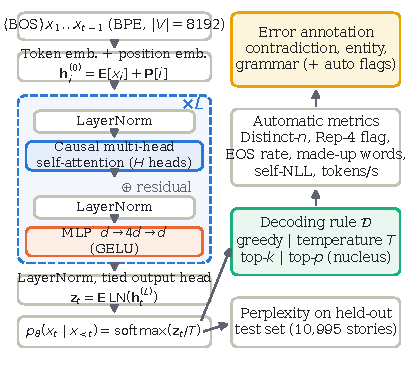
\includegraphics[width=\columnwidth]{fig_architecture}
\caption{Model and study design. Left: pre-LN decoder-only Transformer with causal self-attention and tied output embeddings. Right: the next-token distribution is evaluated by test perplexity and converted to text by a decoding rule $\mathcal{D}$; the text is then scored by automatic metrics and by a rubric-based error annotation.}
\label{fig:arch}
\end{figure}

\subsection{Optimization}
Parameters are updated with AdamW \cite{loshchilov2019adamw} ($\beta_1=0.9$, $\beta_2=0.95$, weight decay $0.1$, gradient-norm clipping at $1.0$). The learning rate follows a linear warm-up for $s_w$ steps and a cosine decay to $\eta_{\min}$,
\begin{equation}
\eta_s = \begin{cases}
\eta_{\max}\, s/s_w, & s< s_w,\\[2pt]
\eta_{\min} + \tfrac{1}{2}(\eta_{\max}-\eta_{\min})\Big(1+\cos\frac{\pi(s-s_w)}{S-s_w}\Big), & s\ge s_w,
\end{cases}
\end{equation}
with $\eta_{\max}=6\times10^{-4}$, $\eta_{\min}=6\times10^{-5}$ and $S$ total steps.

%% ----------------------------------------------------------------------------
\section{Decoding Rules}
\label{sec:decoding}

Given logits $\mathbf{z}_t$, a decoding rule $\mathcal{D}$ chooses $x_t$ and the process repeats until $\EOS$ or a length limit (Algorithm~\ref{alg:decode}). Let $\pi_{(1)}\ge\pi_{(2)}\ge\dots$ denote the next-token probabilities sorted in decreasing order and $v_{(r)}$ the token of rank $r$.

\emph{Greedy decoding} selects the mode,
\begin{equation}
x_t = \argmax_{v\in\mathcal{V}} p_\theta(v\mid\mathbf{x}_{<t}).
\end{equation}

\emph{Temperature sampling} draws from the rescaled distribution
\begin{equation}
q_T(v) = \frac{\exp(z_{t,v}/T)}{\sum_{u\in\mathcal{V}}\exp(z_{t,u}/T)},
\label{eq:temp}
\end{equation}
which is sharper for $T<1$, equals the model distribution for $T=1$ (ancestral sampling) and tends to greedy decoding as $T\to0$.

\emph{Top-$k$ sampling} \cite{fan2018hierarchical} keeps the $k$ most probable tokens, $\mathcal{S}_k=\{v_{(1)},\dots,v_{(k)}\}$.

\emph{Top-$p$ (nucleus) sampling} \cite{holtzman2020curious} keeps the smallest prefix of the sorted vocabulary whose mass reaches $p$,
\begin{equation}
\mathcal{S}_p=\{v_{(1)},\dots,v_{(m)}\},\quad m=\min\Big\{m' : \sum_{r=1}^{m'}\pi_{(r)}\ge p\Big\}.
\label{eq:nucleus}
\end{equation}
For both truncation rules the token is sampled from the renormalized distribution
\begin{equation}
q_{\mathcal{S}}(v) = \frac{p_\theta(v\mid\mathbf{x}_{<t})\,\mathbb{1}[v\in\mathcal{S}]}{\sum_{u\in\mathcal{S}}p_\theta(u\mid\mathbf{x}_{<t})}.
\label{eq:renorm}
\end{equation}
The nucleus size $m$ in (\ref{eq:nucleus}) adapts to the shape of the distribution, while $k$ is fixed. Section~\ref{sec:nucleus} measures how strongly $m$ varies in practice.

\begin{algorithm}[!t]
\caption{Autoregressive generation with a decoding rule}
\label{alg:decode}
\begin{algorithmic}[1]
\Require prompt tokens $\mathbf{x}$ (starting with $\BOS$), model $p_\theta$, rule $\mathcal{D}$, limit $N_{\max}$
\For{$n=1$ \textbf{to} $N_{\max}$}
  \State $\mathbf{z} \gets$ logits of $p_\theta(\cdot\mid\mathbf{x}_{-L_c:})$ at the last position
  \If{$\mathcal{D}$ is greedy} \State $x \gets \argmax_v z_v$
  \Else
    \State $\mathbf{q}\gets\mathrm{softmax}(\mathbf{z}/T)$ \Comment{(\ref{eq:temp})}
    \State $\mathcal{S}\gets$ top-$k$ set, nucleus (\ref{eq:nucleus}), or $\mathcal{V}$
    \State sample $x\sim q_{\mathcal{S}}$ \Comment{(\ref{eq:renorm})}
  \EndIf
  \State append $x$ to $\mathbf{x}$; \textbf{if} $x=\EOS$ \textbf{then break}
\EndFor
\State \Return $\mathbf{x}$
\end{algorithmic}
\end{algorithm}

The following property makes precise why truncation moves generated text toward the high-probability region of the model.

\begin{proposition}
\label{prop:trunc}
Let $\pi$ be a distribution over $\mathcal{V}$ with entropy $H(\pi)=\mathbb{E}_{\pi}[-\log\pi(v)]$, and let $\mathcal{S}$ be any top-mass set, i.e., $\pi(u)\ge\pi(w)$ for all $u\in\mathcal{S}$, $w\notin\mathcal{S}$ (this includes $\mathcal{S}_k$ and $\mathcal{S}_p$). Then the expected surprisal of a token drawn from the renormalized distribution $q_{\mathcal{S}}$, measured under $\pi$, satisfies
\begin{equation}
\mathbb{E}_{v\sim q_{\mathcal{S}}}[-\log\pi(v)] \le H(\pi),
\end{equation}
with equality if and only if $\pi(\mathcal{S})=1$ or all tokens of positive probability have equal probability.
\end{proposition}
\begin{IEEEproof}
Write $P=\pi(\mathcal{S})$, $a=\mathbb{E}_{q_{\mathcal{S}}}[-\log\pi(v)]$ and $b=\mathbb{E}_{\pi(\cdot\mid v\notin\mathcal{S})}[-\log\pi(v)]$ for $P<1$. Since $-\log\pi(u)\le-\log\pi(w)$ for every $u\in\mathcal{S}$ and $w\notin\mathcal{S}$, we have $a\le\max_{u\in\mathcal{S}}(-\log\pi(u))\le\min_{w\notin\mathcal{S}}(-\log\pi(w))\le b$. By the law of total expectation, $H(\pi)=Pa+(1-P)b\ge Pa+(1-P)a=a$. Equality requires $P=1$ or $a=b$, and $a=b$ forces all surprisal values to coincide.
\end{IEEEproof}

Applied at every step, Proposition~\ref{prop:trunc} predicts that text produced by top-$k$ or top-$p$ sampling has a lower negative log-likelihood under the generating model than text produced by ancestral sampling. If the model is well calibrated, ancestral sampling should in turn match the model's cross-entropy on human text. We test both predictions in Section~\ref{sec:selfnll}. The same argument applies to temperatures $T<1$, which move mass toward high-probability tokens.

%% ----------------------------------------------------------------------------
\section{Data and Leakage Control}
\label{sec:data}

TinyStories \cite{eldan2023tinystories} provides a training split of 2,119,719 stories and a validation split of 21,990 stories. Inspection showed three problems: 15\% of the training stories are exact duplicates, 1.2\% are truncated in mid-sentence, and 6,601 validation stories (30.0\%) also occur verbatim in the training split. The last point is a train--test leak that lowers every likelihood-based validation score. We therefore apply the cleaning steps of Table~\ref{tab:cleaning}. Because the validation split is also used to select checkpoints, it is split into two fixed halves (seed 1337): 10,995 stories for validation and 10,995 for a \emph{test} split that is used only for the final scores. The validation text is left unchanged, and the three splits share no story.

\begin{table}[!t]
\centering
\caption{Cleaning of the TinyStories Training Split}
\label{tab:cleaning}
\begin{tabular}{@{}lrr@{}}
\toprule
Step & Stories left & Removed \\
\midrule
Raw training split & 2,119,719 & -- \\
Remove empty stories & 2,119,489 & 230 \\
Remove truncated ($<$20 words or no final punctuation) & 2,094,957 & 24,532 \\
Remove exact duplicates & 1,778,710 & 316,247 \\
Remove stories that occur in validation & \textbf{1,772,187} & 6,523 \\
\bottomrule
\end{tabular}
\end{table}

A byte-level BPE tokenizer \cite{gage1994bpe,sennrich2016bpe} with 8,192 tokens, including $\langle$PAD$\rangle$, $\langle$UNK$\rangle$, $\BOS$ and $\EOS$, is trained on 100,000 cleaned training stories. On the validation split it produces 1.20 tokens per word and no unknown tokens; 85\% of the stories fit into the 256-token context. Every story is encoded as $\BOS$\,story\,$\EOS$, all stories are concatenated, and the stream is cut into non-overlapping windows of 256 tokens whose targets are the inputs shifted by one position. The full training stream contains 372.6M tokens; validation and test contain 2.27M and 2.26M tokens.

%% ----------------------------------------------------------------------------
\section{Experimental Setup}
\label{sec:setup}

\subsection{Models and Training}
Table~\ref{tab:models} lists the two models. The \emph{baseline} is trained on the first 100,000 cleaned stories (20.8M tokens, about two epochs) and the \emph{small} model on all 1,772,187 stories (it sees 164M tokens, i.e., 44\% of the stream, so no story is repeated). Both use dropout 0.1, fp32 arithmetic and random seed 1337, and the checkpoint with the lowest validation loss is kept. All computation runs on one Intel CPU (24 logical cores, 63.7\,GB RAM) with PyTorch 2.14 \cite{paszke2019pytorch} and no GPU.

\begin{table}[!t]
\centering
\caption{Model Configurations and Training Budgets}
\label{tab:models}
\begin{tabular}{@{}lrr@{}}
\toprule
 & Baseline & Small \\
\midrule
Layers $L$ / heads $H$ / width $d$ & 4 / 4 / 256 & 6 / 6 / 384 \\
Context $L_c$ & 256 & 256 \\
Parameters (non-embedding) & 5.32M (3.16M) & 13.89M (10.65M) \\
Training stories & 100,000 & 1,772,187 \\
Effective batch (tokens) & 32 seq.\ (8,192) & 64 seq.\ (16,384) \\
Steps / warm-up steps & 5,000 / 200 & 10,000 / 500 \\
Tokens seen & 41M & 164M \\
Training time (CPU) & 1.0\,h & 9.9\,h \\
Peak training memory & 989\,MB & 1,438\,MB \\
\bottomrule
\end{tabular}
\end{table}

\subsection{Generation Protocol}
Eight story openings serve as prompts (e.g., ``Once upon a time'', ``Tom had a big red ball'', ``Sara found a shiny key''). For every sampling rule we draw five stories per prompt (40 stories); greedy decoding is deterministic and yields one story per prompt (8 stories). Generation stops at $\EOS$ or after $N_{\max}=512$ new tokens, a limit that 98.0\% of human validation stories satisfy. Random seeds are fixed so that every sample can be reproduced.

\subsection{Automatic Metrics}
\emph{Distinct-$n$} \cite{li2016diversity} is the ratio of unique to total $n$-grams in a set of texts $\mathcal{T}$,
\begin{equation}
\mathrm{D}_n(\mathcal{T}) = \frac{|\{g : g\in \mathrm{ngrams}_n(\tau),\ \tau\in\mathcal{T}\}|}{\sum_{\tau\in\mathcal{T}}|\mathrm{ngrams}_n(\tau)|}.
\end{equation}
Because $\mathrm{D}_n$ decreases with the amount of pooled text, it is computed on the first 100 words of each story, in groups that contain exactly one story per prompt, and averaged over groups.

\emph{Repetition.} For a single story $\tau$ with 4-gram list $G_\tau$, the repeated-4-gram rate is
\begin{equation}
\mathrm{Rep}_4(\tau) = 1-\frac{|\mathrm{set}(G_\tau)|}{|G_\tau|}.
\end{equation}
A story is \emph{flagged} as repetitive if $\mathrm{Rep}_4(\tau)>\gamma$, where $\gamma=0.0569$ is the 95th percentile of $\mathrm{Rep}_4$ over the 10,995 human validation stories. By construction, 5\% of human stories are flagged.

\emph{EOS rate} is the fraction of stories that end with $\EOS$ before the limit.

\emph{Made-up-word rate.} Let $\mathcal{W}$ be the set of 23,116 distinct words found in 300,000 cleaned training stories. The non-word rate of a set of texts is
\begin{equation}
\mathrm{MW}(\mathcal{T})=\frac{\#\{\text{word tokens } w\in\mathcal{T}: w\notin\mathcal{W}\}}{\#\{\text{word tokens in }\mathcal{T}\}}.
\end{equation}
Human validation text has $\mathrm{MW}=0.021\%$ (68 of 323,739 words).

\emph{Self-NLL.} To quantify how far a decoding rule moves text toward the mode of the model, we score each generated continuation $\mathbf{y}$ of a prompt $\mathbf{c}$ with the model that produced it,
\begin{equation}
\mathrm{NLL}(\mathbf{y}\mid\mathbf{c}) = -\frac{1}{|\mathbf{y}|}\sum_{t=1}^{|\mathbf{y}|}\log p_\theta(y_t\mid\mathbf{c},\mathbf{y}_{<t}),
\end{equation}
and compare it with the same quantity for 200 human test stories, conditioned on their first five words.

\emph{Speed.} Throughput is measured for 200 generated tokens per rule (three repetitions, 24 threads), and a measurement is accepted only if other processes use at most 15\% of the CPU before and during timing.

\subsection{Error Annotation}
A separate set of 60 stories (top-$p$ sampling, $p=0.90$, the eight prompts) from the small model is annotated with the rubric in Table~\ref{tab:rubric}. A story receives a label if \emph{any} part of it meets the definition, so the rates are strict. Repetition and incompleteness are taken from the automatic flags, and the annotator additionally records whether each repetition flag is a real loop, a false alarm, or a missed loop.

\begin{table}[!t]
\centering
\caption{Error Rubric for Generated Stories}
\label{tab:rubric}
\begin{tabular}{@{}p{0.24\columnwidth}p{0.68\columnwidth}@{}}
\toprule
Error & Definition (one occurrence suffices) \\
\midrule
Contradiction & A statement clashes with an earlier fact of the story or does not follow from it (place, object, event, feeling). \\
Entity consistency & A character changes name, gender or species; appears without introduction in a way that confuses identity; or the wrong character speaks or acts. \\
Grammar & At least one ungrammatical sentence or invented word. \\
Repetition (auto) & $\mathrm{Rep}_4>\gamma$. \\
Incomplete (auto) & No $\EOS$ within $N_{\max}$ tokens, or ends without final punctuation. \\
\bottomrule
\end{tabular}
\end{table}

\subsection{Statistical Analysis}
Proportions are reported with 95\% Wilson intervals \cite{wilson1927probable},
\begin{equation}
\frac{\hat{p}+\frac{z^2}{2n}}{1+\frac{z^2}{n}} \pm \frac{z}{1+\frac{z^2}{n}}\sqrt{\frac{\hat{p}(1-\hat{p})}{n}+\frac{z^2}{4n^2}},\quad z=1.96.
\end{equation}
Means are reported with percentile bootstrap intervals from 5,000 resamples \cite{efron1993bootstrap}. Differences in proportions are tested with the two-sided Fisher exact test, and differences in means with a two-sided pooled-resampling bootstrap test. Monotone association is measured with Spearman's $\rho$ and a permutation test. With 40 stories per setting, only large differences in flag rates can be detected, and we report non-significant results as such.

%% ----------------------------------------------------------------------------
\section{Results}
\label{sec:results}

\subsection{Language-Modeling Quality}
\label{sec:ppl}
The small model reaches a test cross-entropy of 1.7473 nats (perplexity 5.74) and the baseline 2.2700 nats (perplexity 9.68), a 41\% reduction in perplexity on the same tokenizer and test stories. Validation and test agree closely (1.7467 vs.\ 1.7473 for the small model, 2.2705 vs.\ 2.2700 for the baseline), so checkpoint selection on validation did not bias the results. Fig.~\ref{fig:curves} plots the learning curves against the number of training tokens. Validation loss decreases at every evaluation and stays slightly below the training loss (dropout is active only in training), so neither model overfits. At an equal budget of 41M tokens, the small model's validation loss is 2.10 against 2.27 for the baseline, which shows the advantage of the larger model independently of the larger budget. At the end of training, the small model was still improving slowly (1.778 to 1.774 over the last 500 steps).

\begin{figure}[!t]
\centering
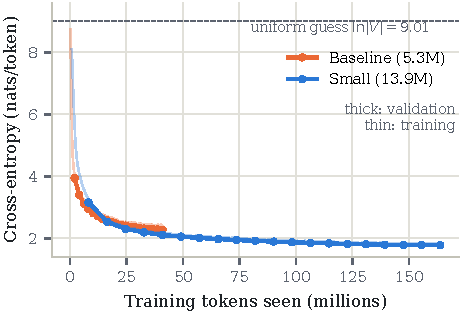
\includegraphics[width=\columnwidth]{fig_learning_curves}
\caption{Training (thin) and validation (thick) cross-entropy versus training tokens. The dashed line is the loss of a uniform prediction over 8,192 tokens.}
\label{fig:curves}
\end{figure}

\subsection{Effect of the Decoding Rule}
\label{sec:dec}
Table~\ref{tab:decoding} reports all automatic metrics, and Fig.~\ref{fig:tradeoff} places each rule in the diversity--repetition plane together with human stories.

\begin{table*}[!t]
\centering
\caption{Decoding Results (40 Stories per Sampling Rule, 8 for Greedy). Rep$_4$: Mean Repeated-4-Gram Rate with 95\% Bootstrap Interval. Flagged: Stories Above the Human 95th Percentile. MW: Made-Up-Word Rate. Human Stories: 10,995 Validation Stories (MW on 2,000).}
\label{tab:decoding}
\setlength{\tabcolsep}{4.2pt}
\begin{tabular}{@{}llccccccc@{}}
\toprule
Model & Rule & D$_1$ & D$_2$ & Rep$_4$ (\%) [95\% CI] & Flagged & EOS (\%) & MW (\%) & Tokens/s \\
\midrule
\multicolumn{2}{@{}l}{Human stories} & 0.331 & 0.764 & 1.64 & 5\% (def.) & -- & 0.021 & -- \\
\midrule
\multirow{7}{*}{\shortstack[l]{Baseline\\(5.3M)}}
 & Greedy      & 0.151 & 0.391 & 48.85 [33.0, 66.5] & 8/8   & 75.0  & 0.000 & 366 \\
 & $T=0.7$     & 0.263 & 0.655 & 5.07 [3.30, 7.14]  & 12/40 & 87.5  & 0.000 & 332 \\
 & $T=1.0$     & 0.358 & 0.799 & 0.56 [0.36, 0.77]  & 0/40  & 97.5  & 0.408 & 344 \\
 & $k=20$      & 0.297 & 0.739 & 1.80 [1.13, 2.59]  & 2/40  & 90.0  & 0.000 & 346 \\
 & $k=50$      & 0.322 & 0.768 & 1.61 [1.08, 2.19]  & 1/40  & 87.5  & 0.038 & 341 \\
 & $p=0.90$    & 0.310 & 0.738 & 1.60 [1.20, 2.03]  & 1/40  & 92.5  & 0.042 & 279 \\
 & $p=0.95$    & 0.336 & 0.782 & 1.27 [0.88, 1.71]  & 0/40  & 95.0  & 0.070 & 266 \\
\midrule
\multirow{7}{*}{\shortstack[l]{Small\\(13.9M)}}
 & Greedy      & 0.238 & 0.586 & 16.20 [5.36, 29.9] & 6/8   & 87.5  & 0.000 & 161 \\
 & $T=0.7$     & 0.275 & 0.693 & 4.31 [3.03, 5.72]  & 10/40 & 92.5  & 0.014 & 160 \\
 & $T=1.0$     & 0.334 & 0.777 & 1.27 [0.84, 1.77]  & 1/40  & 100.0 & 0.337 & 154 \\
 & $k=20$      & 0.298 & 0.733 & 2.70 [1.95, 3.59]  & 3/40  & 95.0  & 0.050 & 155 \\
 & $k=50$      & 0.298 & 0.726 & 2.43 [1.72, 3.17]  & 4/40  & 92.5  & 0.000 & 162 \\
 & $p=0.90$    & 0.303 & 0.738 & 2.95 [1.97, 4.10]  & 4/40  & 92.5  & 0.000 & 145 \\
 & $p=0.95$    & 0.312 & 0.742 & 2.59 [1.72, 3.67]  & 1/40  & 92.5  & 0.039 & 141 \\
\bottomrule
\end{tabular}
\end{table*}

\begin{figure}[!t]
\centering
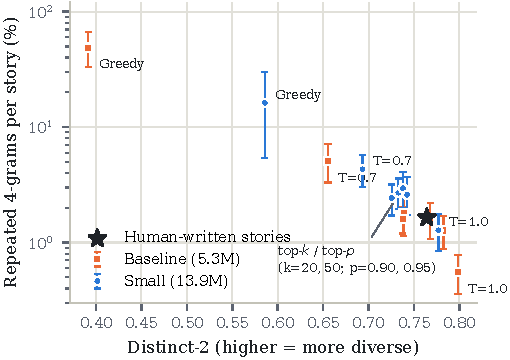
\includegraphics[width=\columnwidth]{fig_tradeoff}
\caption{Diversity (Distinct-2) versus repetition (mean repeated-4-gram rate, log scale, 95\% bootstrap intervals) for each decoding rule and model. The star marks human-written stories. Top-$k$ and top-$p$ rules form a cluster close to the human reference.}
\label{fig:tradeoff}
\end{figure}

\emph{Maximization causes degeneration.} Greedy decoding produces the most repetitive and least diverse text for both models: 48.9\% of the 4-grams of a baseline greedy story are repeats (16.2\% for the small model), and all eight baseline greedy stories are flagged. Typical loops in greedy and low-temperature output repeat a whole sentence (``You are not nice. You are not nice.''). The larger model degenerates less but still loops in six of eight stories. Lowering the temperature to 0.7 has a weaker version of the same effect: 25\% of the small model's stories are flagged, significantly more than with top-$p$ 0.95 (10/40 vs.\ 1/40, Fisher $p=0.007$).

\emph{Pure sampling is diverse but lexically invalid.} With $T=1.0$, Distinct-2 (0.777 small, 0.799 baseline) reaches or exceeds the human value of 0.764, repetition is at or below the human level, and every story of the small model ends with $\EOS$. On these metrics alone, $T=1.0$ would be judged best. However, its made-up-word rate is 0.337\% for the small model and 0.408\% for the baseline, i.e., 16 and 19 times the human rate, and significantly higher than with top-$p$ 0.95 (24/7,124 vs.\ 3/7,729 words, $p=1.7\times10^{-5}$). Examples are ``oripped'', ``alreadypow'' and ``neverld''. Distinct-$n$ counts each such non-word as additional diversity, so it rewards exactly the failure that sampling from the unreliable tail produces.

\emph{Truncated sampling is close to human statistics.} Top-$k$ and top-$p$ rules form a tight cluster (Distinct-2 0.726--0.742 for the small model) with repetition between the greedy and $T=1.0$ extremes and non-word rates at most 0.05\%. Within the cluster the differences in flag rates are not statistically significant at $n=40$ (e.g., top-$p$ 0.90 vs.\ 0.95: 4/40 vs.\ 1/40, $p=0.36$). We select top-$p$ with $p=0.95$ as the default rule because it is the only setting without a weak point: the lowest flag rate of the truncated rules, Distinct-2 closest to human text, and a non-word rate within twice the human rate.

\emph{Model size interacts with truncation.} Under the same truncation rule, the larger model repeats \emph{more} than the baseline: the mean Rep$_4$ is higher for top-$p$ 0.90 (2.95\% vs.\ 1.60\%, bootstrap $p=0.026$), top-$p$ 0.95 (2.59\% vs.\ 1.27\%, $p=0.019$) and $T=1.0$ (1.27\% vs.\ 0.56\%, $p=0.008$), while the differences for top-$k$ and $T=0.7$ are not significant ($p\ge0.087$). The flag rates show the same direction but are not individually significant. In the separate 60-story annotation set, however, 13 small-model stories are flagged against 2 baseline stories ($p=0.004$). We attribute this to sharper next-token distributions: a better model concentrates mass on fewer tokens, so the nucleus for a fixed $p$ becomes smaller and decoding becomes more mode-seeking. Reading the stories supports this interpretation. The baseline repeats less partly because its text is looser and contains more broken phrases, so exact 4-grams recur less often. Section~\ref{sec:selfnll} gives a direct measurement.

\subsection{Likelihood of Generated Text}
\label{sec:selfnll}
Fig.~\ref{fig:selfnll} shows the self-NLL of the generated continuations. Both predictions of Proposition~\ref{prop:trunc} hold. First, every truncated or cooled rule yields text that the model finds much more probable than human text. For the small model the self-NLL is 0.54 nats/token for greedy decoding, 0.92 for $T=0.7$, 1.29--1.36 for top-$k$ and 1.20--1.30 for top-$p$, compared with 1.72 [1.66, 1.78] for human test stories. Second, ancestral sampling ($T=1.0$) gives 1.76 [1.65, 1.88], statistically indistinguishable from the human value, which indicates that the small model is well calibrated in the aggregate. For the baseline the same pattern holds at a higher level (human 2.27, $T=1.0$ 2.40). The human values agree with the test cross-entropies of Section~\ref{sec:ppl} (1.75 and 2.27).

The self-NLL of each model's own truncated output is lower for the small model (top-$p$ 0.95: 1.30 vs.\ 1.93). Measured relative to human text, the small model's top-$p$ 0.95 output lies 0.41 nats/token below the human level and the baseline's 0.34 nats/token below, which is consistent with the stronger mode-seeking behavior and the higher repetition reported above.

\begin{figure}[!t]
\centering
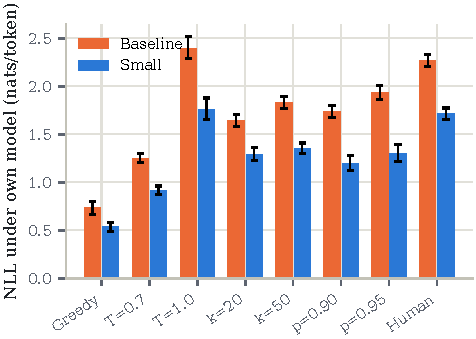
\includegraphics[width=\columnwidth]{fig_self_nll}
\caption{Negative log-likelihood (nats/token) of generated continuations under the model that generated them, with 95\% bootstrap intervals; ``Human'' is 200 test stories under the same model. Only ancestral sampling ($T=1.0$) reaches the human level, as predicted by Proposition~\ref{prop:trunc}.}
\label{fig:selfnll}
\end{figure}

\subsection{Why a Fixed $k$ Mis-Truncates}
\label{sec:nucleus}
Running the small model over 100 human test stories (18,394 positions) shows how much the shape of the next-token distribution varies (Fig.~\ref{fig:nucleus}). The nucleus for $p=0.90$ has a median size of 5 tokens, but its 10th and 90th percentiles are 1 and 54 tokens. In 20.7\% of the positions a single token already carries 90\% of the mass, so top-$k$ with $k=20$ adds 19 tokens from the tail exactly where the model is confident. Conversely, in 21.8\% of the positions the 20 most probable tokens hold less than 90\% of the mass (10.9\% for $k=50$), so top-$k$ removes plausible continuations exactly where the model is uncertain. For $p=0.95$ the median nucleus has 8 tokens and the 90th percentile 142. This variability explains why the fixed-$k$ rules admitted non-words (0.050\% for $k=20$ in the small model) while top-$p$ 0.90 admitted none, and it supports adaptive truncation for small models.

\begin{figure}[!t]
\centering
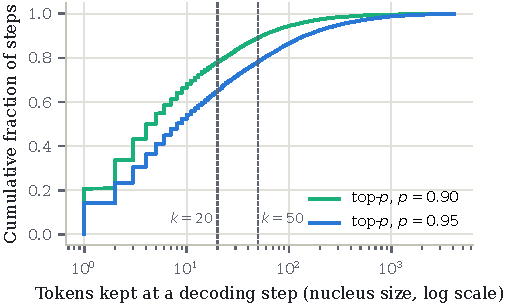
\includegraphics[width=\columnwidth]{fig_nucleus}
\caption{Cumulative distribution of the nucleus size (\ref{eq:nucleus}) of the small model over 18,394 positions of human test stories. Dashed lines mark the fixed sizes of top-$k$ sampling.}
\label{fig:nucleus}
\end{figure}

\subsection{Error Analysis}
\label{sec:errors}
Fig.~\ref{fig:errors} summarizes the annotation of 60 small-model stories. Contradictions are the most frequent error (53/60, 88\%, 95\% CI [78, 94]), followed by entity inconsistency (33/60, 55\% [43, 67]) and grammatical errors (22/60, 37\% [26, 49]). The automatic flags mark 13 stories as repetitive (22\%) and 4 as incomplete (7\%). Only 5 stories (8\%) are free of all three annotated error types; 14 have one type, 29 two and 12 all three.

\begin{figure*}[!t]
\centering
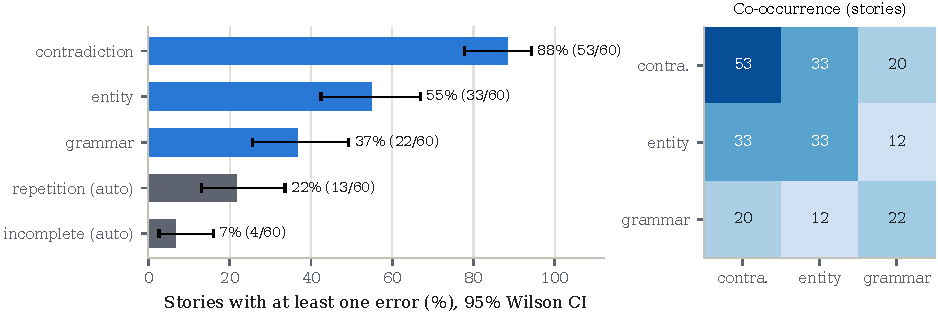
\includegraphics[width=0.92\textwidth]{fig_errors}
\caption{Error analysis of 60 stories from the small model (top-$p$, $p=0.90$). Left: share of stories with each error type and 95\% Wilson intervals; blue bars are annotated, grey bars are automatic flags. Right: number of stories that contain both error types.}
\label{fig:errors}
\end{figure*}

\emph{The errors are discourse-level.} Most individual sentences are grammatical, yet the model loses track of who is who and what is where over the course of a story. Recurrent patterns include (i) the same noun phrase for two characters (``The cat was happy to see the cat''); (ii) ownership that flips between characters (Tom's ball becomes Sue's); (iii) objects that turn into other objects (a key becomes a penny, then a coin); (iv) the wrong speaker (``Lily said, `My name is Max' ''); and (v) characters who appear without introduction. Entity errors never occur alone in our sample: all 33 stories with an entity error also contain a contradiction, and 20 of the 22 stories with a grammatical error do as well (Fig.~\ref{fig:errors}, right). This co-occurrence is consistent with a single underlying weakness, namely the limited ability to maintain a coherent state of the story, rather than three independent failure modes.

\emph{Errors accumulate with length.} The number of annotated error types per story correlates with story length (Spearman $\rho=0.34$, permutation $p=0.008$). Stories at or above the median length of 176 words contain 2.1 error types on average, compared with 1.5 for shorter stories (bootstrap $p=0.007$). All four incomplete stories reached the 512-token limit rather than ending badly, and they are also among the most repetitive: once a small model loses the plot, it tends to continue indefinitely instead of ending the story.

\emph{Validity of the automatic repetition flag.} Of the 13 flagged stories, 11 contain a real loop (e.g., ``I'm sorry, dad.'' three times) and 2 are false alarms: one very short story, and one in which every animal is called ``the cat'', so that an entity error produces repeated 4-grams. Three mild loops were missed. The flag therefore has a precision of 0.85 and a recall of 0.79 with respect to the annotation, which supports its use as a screening metric. The second false alarm also shows that the categories interact.

\emph{Prompt effects.} The mean number of error types per story ranges from 1.13 (``Once upon a time'') to 2.29 (``Sara found a shiny key'', ``Ben and his mom went to the park''). One prompt is defective: after ``In a small house near the forest'' the model assigns 83.5\% probability to a period, because the phrase usually ends a sentence in the corpus. All seven annotated stories with this prompt therefore begin without a protagonist. We kept the prompt to preserve comparability between models and recommend ``In a small house near the forest, there lived'' for future work.

\subsection{Efficiency}
\label{sec:efficiency}
Training the small model took 9.9\,h at about 4,500 tokens/s with a peak memory of 1.4\,GB, and the baseline 1.0\,h (Table~\ref{tab:models}). For generation, the small model needs 1.42\,s for a 200-token story with top-$p$ 0.95 (141 tokens/s) and the baseline 0.75\,s (266 tokens/s); peak evaluation memory is 941\,MB and 781\,MB. Nucleus sampling requires sorting the vocabulary at every step and is therefore slower than top-$k$: 13\% for the small model (141 vs.\ 162 tokens/s) and 22\% for the baseline (266 vs.\ 341 tokens/s), where the sort is a larger share of the per-token cost. Relative to the quality difference, this overhead is small for interactive use.

%% ----------------------------------------------------------------------------
\section{Discussion}
\label{sec:discussion}

\emph{Decoding fixes surface degeneration, not consistency.} Across seven rules, the decoding choice changes repetition by more than an order of magnitude and the non-word rate by a factor of almost twenty, but in no setting does the small model keep the facts of a story consistent. The annotation locates the remaining errors at the discourse level, and Proposition~\ref{prop:trunc} with the self-NLL measurements explains the trade-off: truncation removes the unreliable tail (fewer non-words) at the cost of mode-seeking (more repetition), while no rule can supply story-level state that the model does not represent.

\emph{Diversity metrics need a validity check.} Distinct-$n$ was highest exactly for the rule with the most non-words. We therefore recommend reporting a lexical-validity measure, such as the made-up-word rate, and calibrating repetition thresholds on human text, as done here, whenever diversity is reported for small models.

\emph{Truncation should adapt to the model.} The nucleus size varies by two orders of magnitude across positions, and a better model produces sharper distributions and, under a fixed $p$, more repetition. Adaptive or information-based rules \cite{meister2023typical,hewitt2022truncation} are therefore a promising direction for small models.

\emph{Data hygiene matters for small-model benchmarks.} Since 30.0\% of the official TinyStories validation stories occur in the training split, validation scores computed on the uncleaned split partly measure memorization. We recommend deduplication and an overlap-free held-out split as standard practice.

\emph{Practical recommendation.} For small story models we recommend top-$p$ sampling with $p\approx0.95$, an EOS-terminated length limit well above the typical story length, and evaluation that combines perplexity on a leakage-free split, calibrated repetition, a non-word rate and a discourse-level error audit.

\subsection{Limitations and Threats to Validity}
The study has several limitations. (i) Each model was trained once (seed 1337), so seed variance is not estimated. (ii) Eight prompts and 40 stories per rule limit statistical power, and several differences in flag rates are not significant. (iii) The 60 stories were annotated by a single annotator, with the assistance of a large language model, and have not yet been verified by an independent second annotator, so inter-annotator agreement (e.g., Cohen's $\kappa$ \cite{cohen1960kappa}) cannot be reported; the rates should be read with an uncertainty of roughly $\pm10$ percentage points beyond the sampling intervals. (iv) Only the small model's stories were annotated by hand, so the comparison of error types between model sizes relies on automatic flags. (v) The corpus is synthetic English for young children, and the results may not transfer to other genres or languages. (vi) Speed was measured on a shared desktop CPU, where other processes used 12--15\% of the CPU during timing. Addressing (i)--(iv) is the most direct way to strengthen the conclusions.

%% ----------------------------------------------------------------------------
\section{Conclusion}
\label{sec:conclusion}
We trained two small autoregressive Transformer language models (5.3M and 13.9M parameters) from scratch on a leakage-controlled TinyStories corpus using only a CPU, and studied how seven decoding rules affect their stories and which errors remain. The larger model reduced test perplexity from 9.68 to 5.74. Greedy and low-temperature decoding cause degeneration, pure sampling produces non-words that diversity metrics reward, and truncated sampling, in particular top-$p$ with $p=0.95$, is closest to human statistics. A short proof and a likelihood analysis show why truncation trades tail errors for mode-seeking, and a measurement of nucleus sizes shows why fixed-$k$ truncation is poorly matched to small models. Even with the best rule, 88\% of stories contain a contradiction and 55\% an entity inconsistency, while only 37\% contain a grammatical error: small models are fluent but inconsistent. Future work will add seeds, prompts and independent annotators, evaluate adaptive decoding rules, and use the 13.9M-parameter model as a teacher for knowledge distillation \cite{hinton2015distilling} into smaller students.

%% ----------------------------------------------------------------------------
\section*{Data and Code Availability}
The training and evaluation code, configurations, the trained teacher checkpoint, all generated samples, the error annotations and the script that produces every statistic and figure of this article (\texttt{analysis/paper\_analysis.py}) will be released at [repository URL] upon publication.

\section*{Acknowledgment}
[Funding information.] The authors used an AI assistant (Claude, Anthropic) to help implement the software, produce the first pass of the error annotation, and draft and edit parts of this manuscript. All content was reviewed by the authors, who take full responsibility for it.

\bibliographystyle{IEEEtran}
\bibliography{references}

\end{document}
